% Copyright (c) 2016 Ongun Kanat <ongun.kanat@gmail.com>
% This document is a free software licensed under MIT license.
% For redistribution details look at COPYING file.

% 12pt and ISO A4 paper with title page add notitlepage for otherwise
\documentclass[a4paper, 12pt, titlepage]{article}

% 2cm margin from all sides
\usepackage[a4paper,margin=2cm]{geometry}

% Use American English for dates etc.
\usepackage[american]{babel}
% If document is in Turkish then use
% \usepackage[turkish]{babel}
% or for both
% \usepackage[turkish,american]{babel}

% Indent at section beginnings
% \usepackage{indentfirst} % look at below for reverse
% Paragraph spacings set parindent to 0
\setlength{\parindent}{0pt}
\setlength{\parskip}{12pt}

% utf-8 support
\usepackage[utf8]{inputenc}

% Graphics for PDFTeX
\usepackage[pdftex]{graphicx}

% Figure placement
\usepackage{float}

% An enumeration package for flexible enumeration
\usepackage{enumitem}

% Courier monospace font
\usepackage{courier}

% Links, both local and external
\usepackage{hyperref}
\hypersetup{
	unicode=true,
	colorlinks=true,
	urlcolor=blue,
	citecolor=black,
	menucolor=black,
	linkcolor=black
}

% Figure captions are bold
\usepackage[labelfont=bf]{caption}

% Pseudocode
\usepackage{algorithmicx}
\usepackage{algpseudocode}
\usepackage{algorithm}

% Syntax highlighting simple
\usepackage{listings}
\lstset{basicstyle=\ttfamily,frame=lines,tabsize=4}
\renewcommand{\lstlistingname}{Code}

% Syntax higlighting (advanced)
%\usepackage{minted}

% Title, author and date info
\title{BLG 335E \\ Homework 2 \\ Report}
\author{İbrahim Ethem Göze - 150190054}
\date{December 4\textsuperscript{th}, 2022}

\begin{document}
% Fix Turkish fix hypenation
%\shorthandoff{=}

% For a generic title page one can use standard \maketitle command
% It will use the title info above
% \maketitle

% The title page can be made by hand as below
\begin{titlepage}
	\begin{center}
		\large{Istanbul Technical University \\ Faculty of Computer and Informatics \\ Computer Engineering Department} \\
		\vspace{150pt}
		\Large{BLG 335E \\ Homework 2 \\ Report}  \\
		\vspace{30pt}
		\large{İbrahim Ethem Göze - 150190054} \\
		\vspace{\fill} % Fill out until the page end
		\large{December 4\textsuperscript{th}, 2022}
	\end{center}
\end{titlepage}
\pagenumbering{roman}
\newpage
\tableofcontents
\newpage

% For the ones who doesn't know: 1,2,..9 called West Arabic numbers
\pagenumbering{arabic}
\section{Introduction}
The code is for finding a data set's mean, standard deviation, minimum and maximum value, first and third quartile, and median efficiently.

\section{Algorithms Explained}
\paragraph{}
I used a vector if necessary and sorted it with insertion sort. If the program asked only minimum and maximum value I did not create a vector. Instead I held those values in global variables. If any of mean, standard deviation, first quartile, third quartile or median asked then I created a vector.
\subsection{Insertion Sort}
\par
I used insertion sort because we needed to sort the values again and again. After some point only a couple of elements needs to get sorted. So insertion sort has almost O(n) complexity in this situation. I even stored the size of the vector last time I sorted it and started the next sorting after that point to save more time. 

\newpage

\vspace{150pt}



\newpage

\section{Images and Figures}
I did not include output times for finding the maximum value because it was almost identical with finding the minimum value. Similarly finding firstq and thirdq are very similar with finding median so, I did not include them to. 
\subsection{Mean Time Diagrams}
\begin{figure}[H]
	\centering
	\caption{Mean 10}
	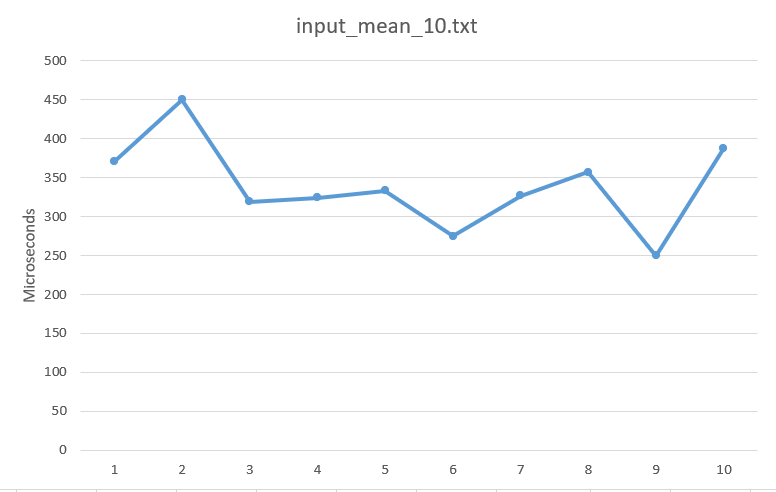
\includegraphics[width=.75\textwidth]{mean10.png} % scale 75%
\end{figure}

\begin{figure}[H]
	\centering
	\caption{Mean 100}
	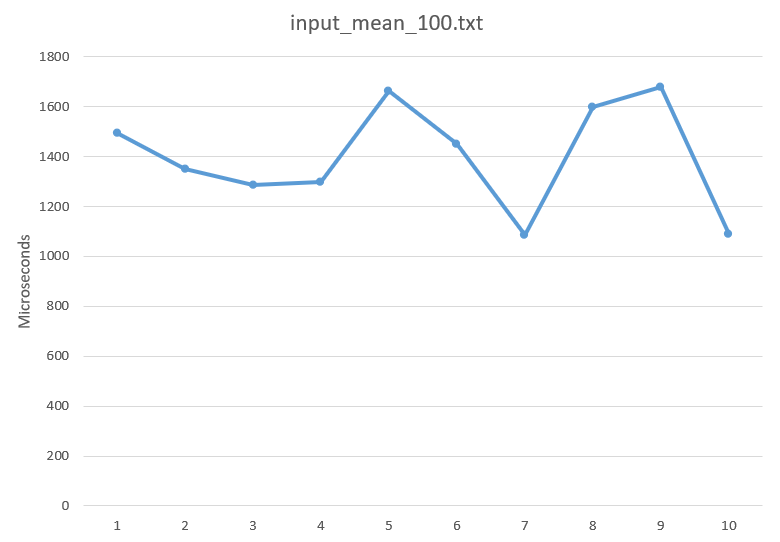
\includegraphics[width=.75\textwidth]{mean100.png} % scale 75%
\end{figure}

\begin{figure}[H]
	\centering
	\caption{Mean 1000}
	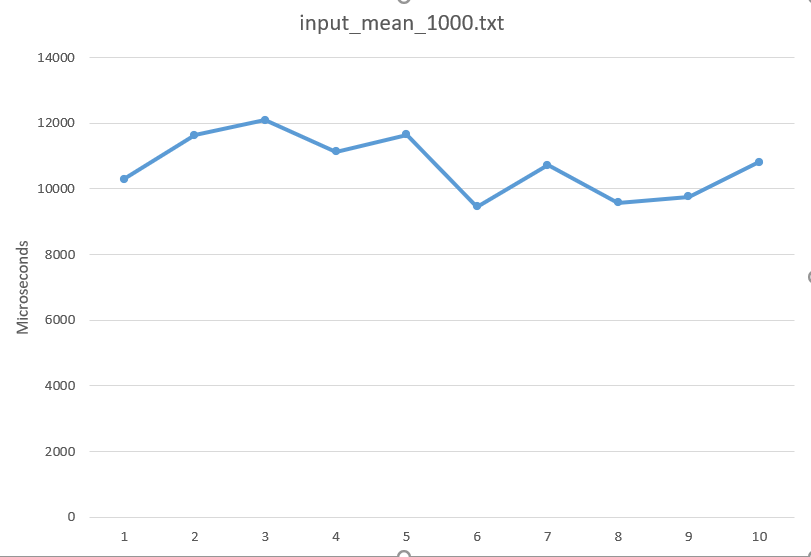
\includegraphics[width=.75\textwidth]{mean1000.png} % scale 75%
\end{figure}

\begin{figure}[H]
	\centering
	\caption{Mean 10000}
	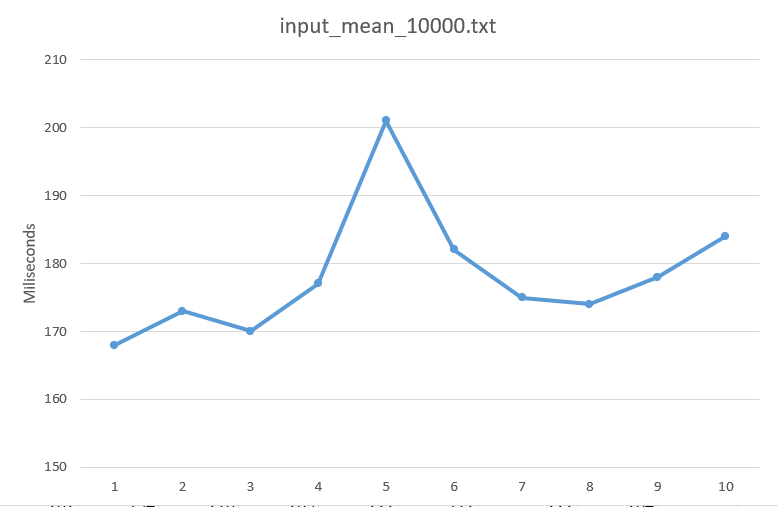
\includegraphics[width=.75\textwidth]{mean10000.png} % scale 75%
\end{figure}

\begin{figure}[H]
	\centering
	\caption{Mean 100000}
	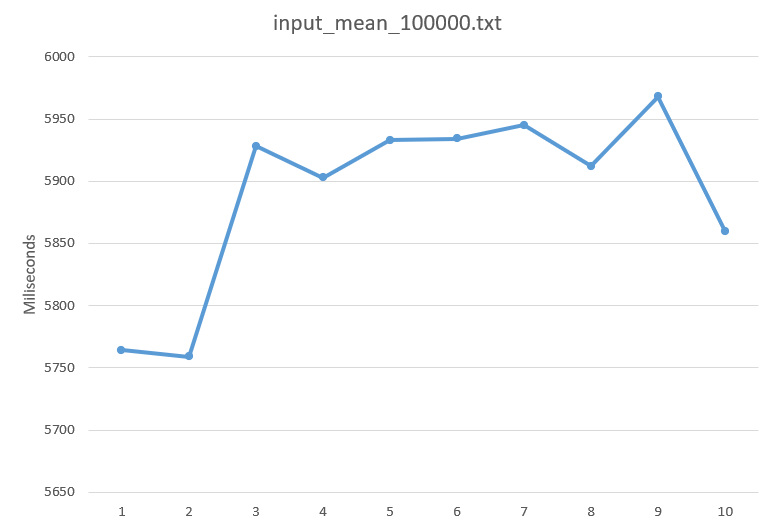
\includegraphics[width=.75\textwidth]{mean100000.png} % scale 75%
\end{figure}

\subsection{Standard Deviation Time Diagrams}
\begin{figure}[H]
	\centering
	\caption{Std 10}
	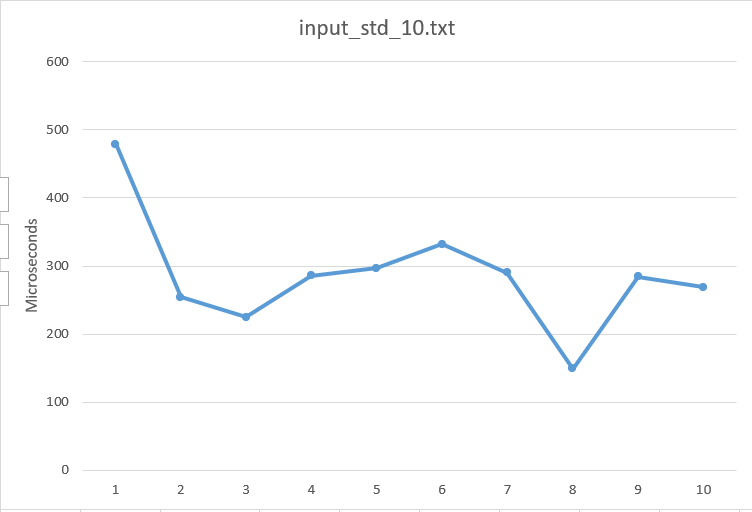
\includegraphics[width=.75\textwidth]{std10.png} % scale 75%
\end{figure}

\begin{figure}[H]
	\centering
	\caption{Std 100}
	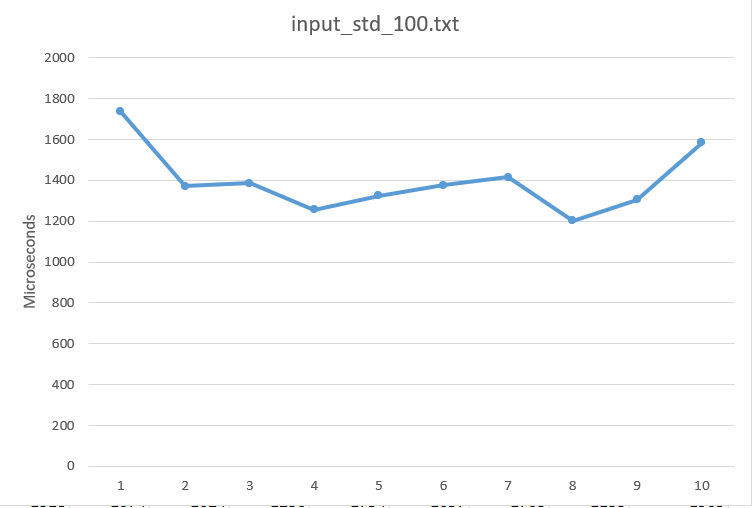
\includegraphics[width=.75\textwidth]{std100.png} % scale 75%
\end{figure}

\begin{figure}[H]
	\centering
	\caption{Std 1000}
	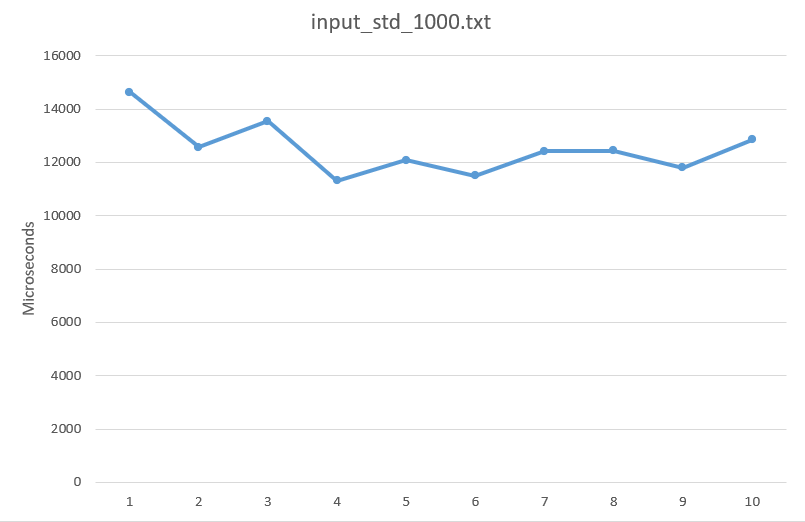
\includegraphics[width=.75\textwidth]{std1000.png} % scale 75%
\end{figure}

\begin{figure}[H]
	\centering
	\caption{Std 10000}
	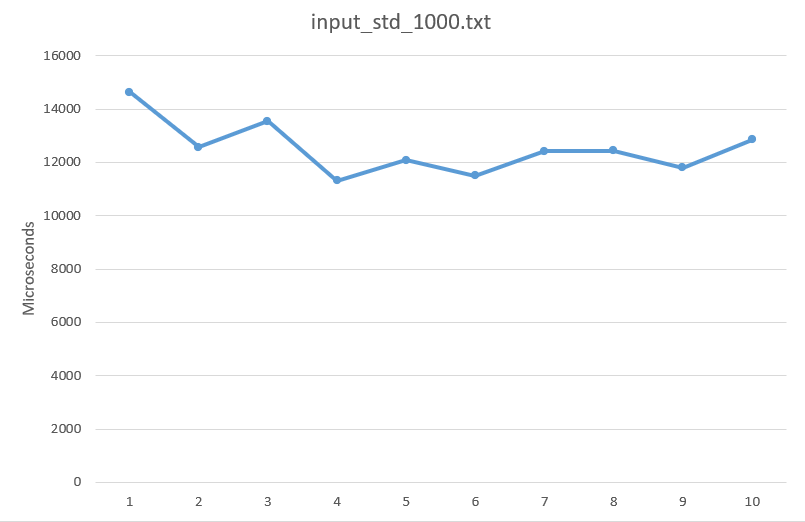
\includegraphics[width=.75\textwidth]{std1000.png} % scale 75%
\end{figure}

\begin{figure}[H]
	\centering
	\caption{Std 100000}
	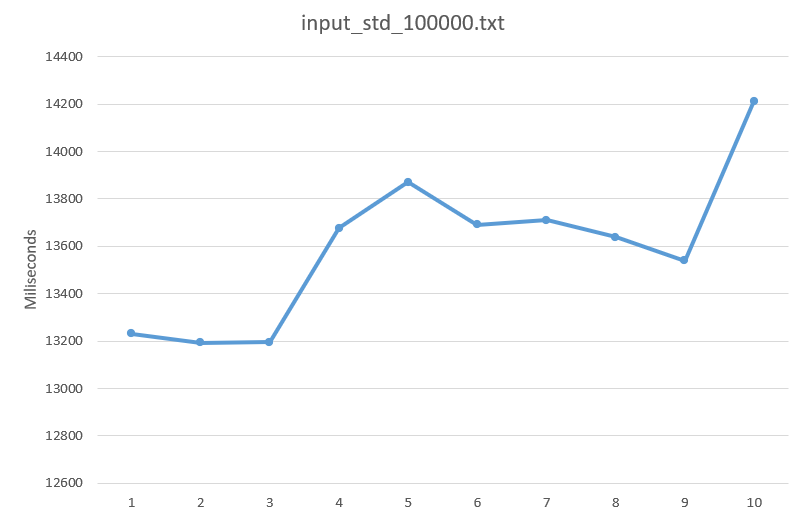
\includegraphics[width=.75\textwidth]{std100000.png} % scale 75%
\end{figure}

\subsection{Minimum Value Time Diagrams}

\begin{figure}[H]
	\centering
	\caption{Min 10}
	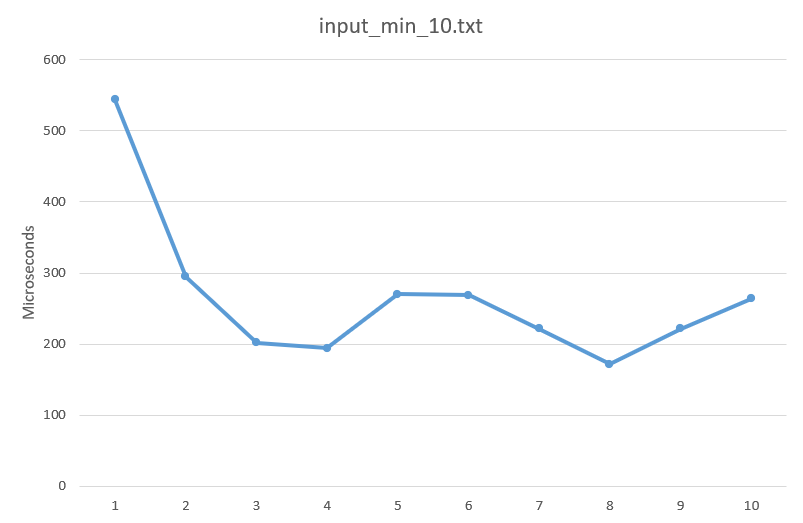
\includegraphics[width=.75\textwidth]{min10.png} % scale 75%
\end{figure}

\begin{figure}[H]
	\centering
	\caption{Min 100}
	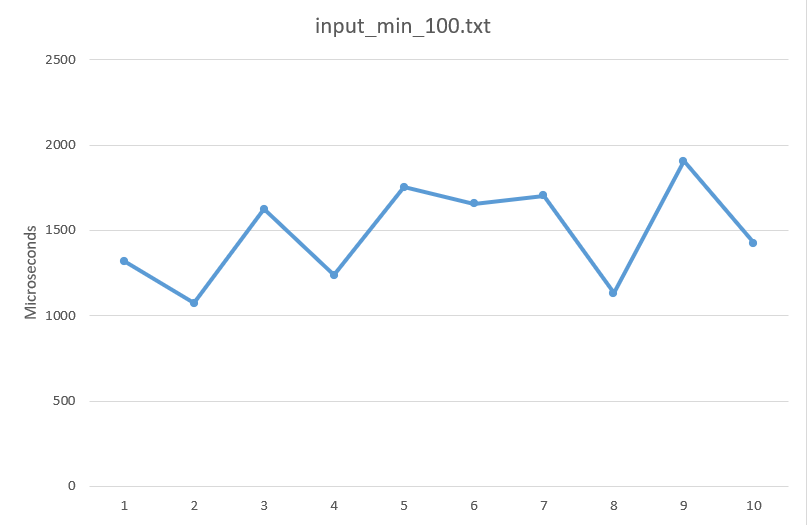
\includegraphics[width=.75\textwidth]{min100.png} % scale 75%
\end{figure}

\begin{figure}[H]
	\centering
	\caption{Min 1000}
	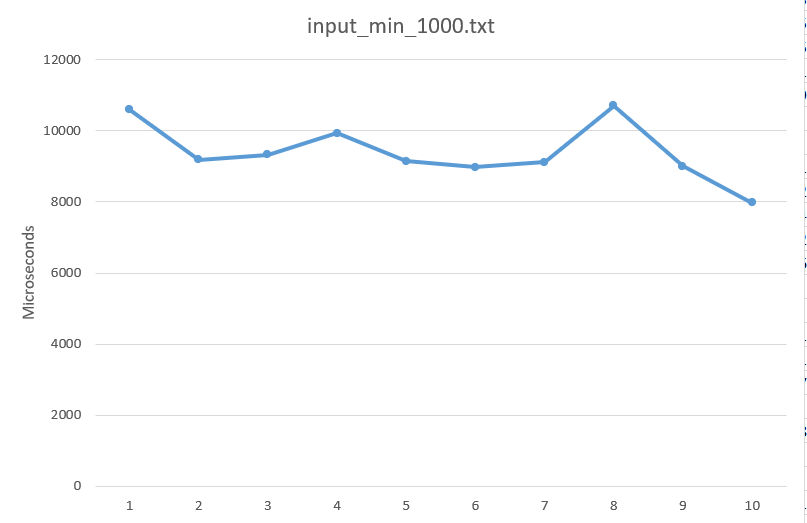
\includegraphics[width=.75\textwidth]{min1000.png} % scale 75%
\end{figure}

\begin{figure}[H]
	\centering
	\caption{Min 10000}
	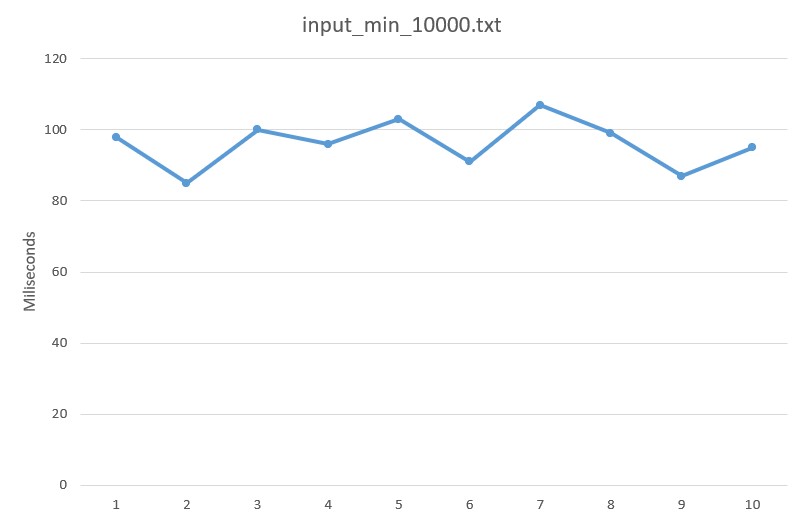
\includegraphics[width=.75\textwidth]{min10000.png} % scale 75%
\end{figure}

\begin{figure}[H]
	\centering
	\caption{Min 100000}
	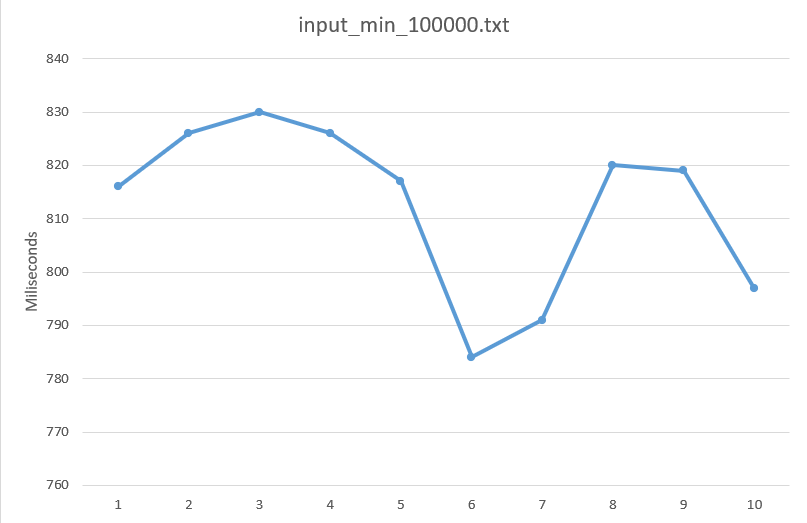
\includegraphics[width=.75\textwidth]{min100000.png} % scale 75%
\end{figure}

\subsection{Median Time Diagrams}

\begin{figure}[H]
	\centering
	\caption{Median 10}
	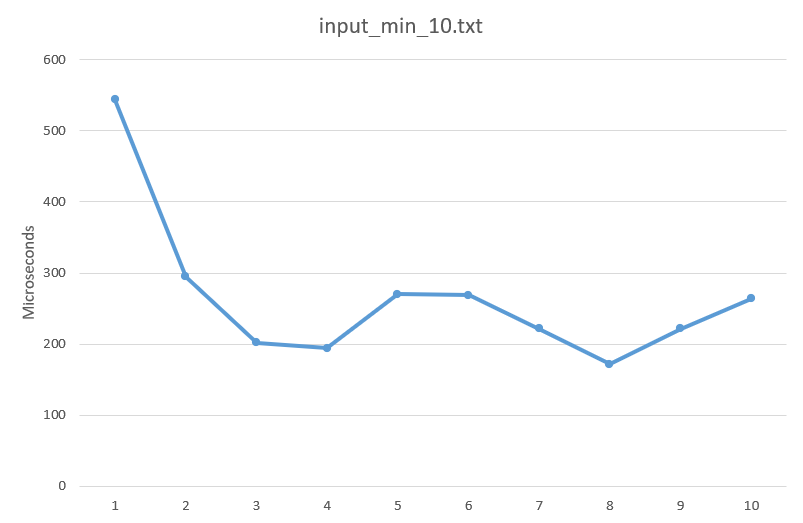
\includegraphics[width=.75\textwidth]{min10.png} % scale 75%
\end{figure}

\begin{figure}[H]
	\centering
	\caption{Median 100}
	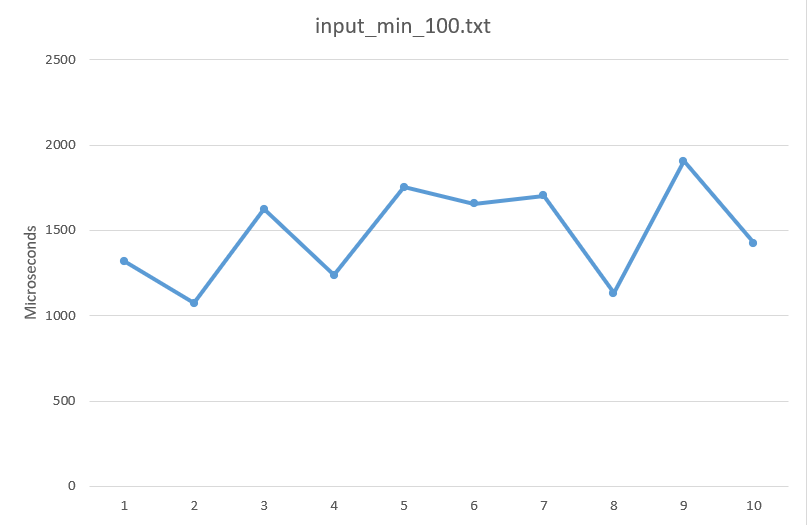
\includegraphics[width=.75\textwidth]{min100.png} % scale 75%
\end{figure}

\begin{figure}[H]
	\centering
	\caption{Median 1000}
	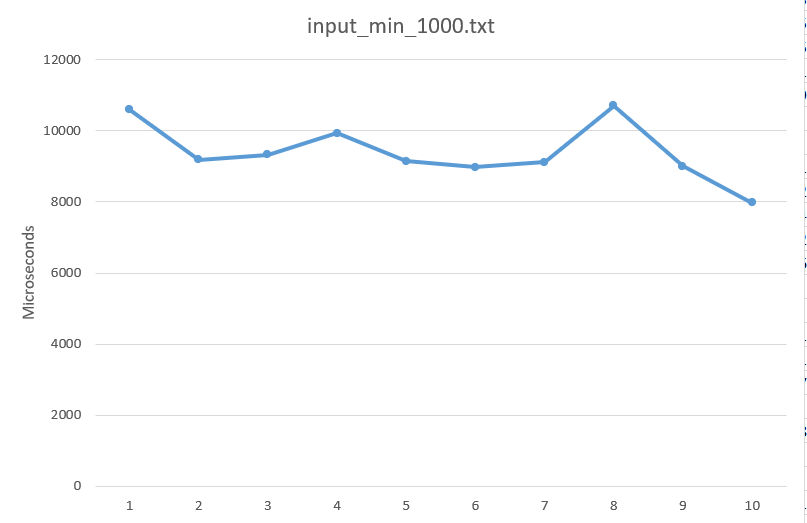
\includegraphics[width=.75\textwidth]{min1000.png} % scale 75%
\end{figure}

\begin{figure}[H]
	\centering
	\caption{Median 10000}
	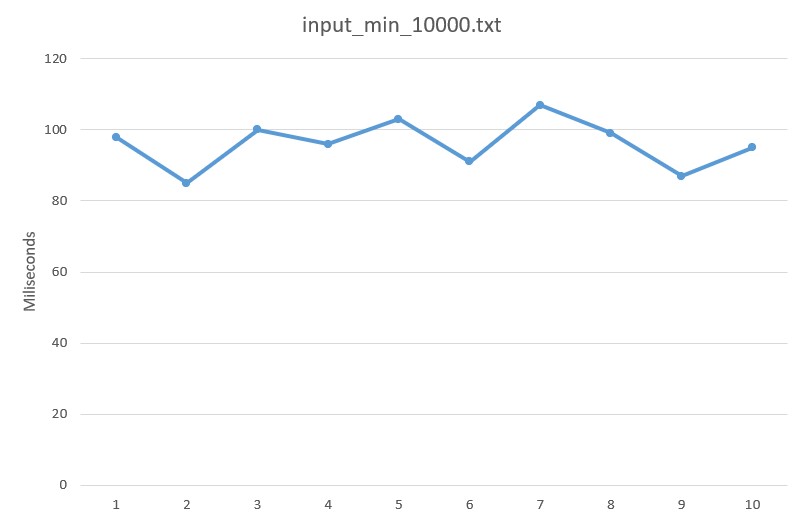
\includegraphics[width=.75\textwidth]{min10000.png} % scale 75%
\end{figure}

\begin{figure}[H]
	\centering
	\caption{Median 100000}
	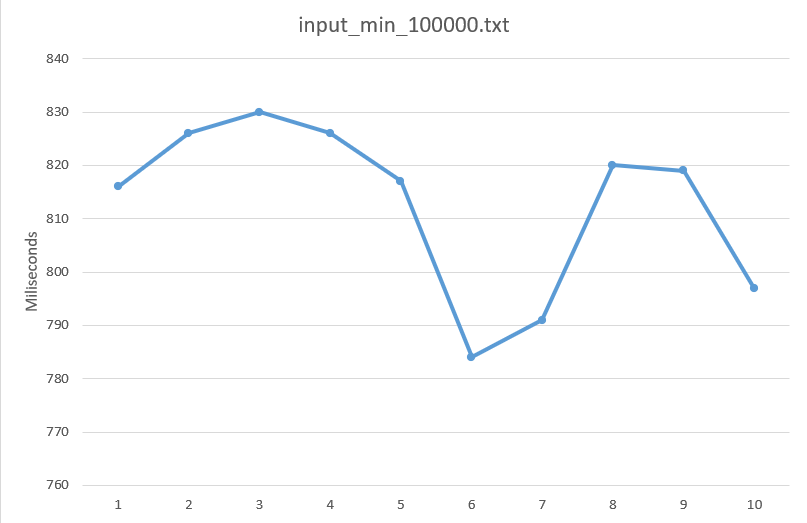
\includegraphics[width=.75\textwidth]{min100000.png} % scale 75%
\end{figure}

\newpage

\section{Inserting Code Pieces}

\subsection{Real Code}

\begin{lstlisting}language=C++,caption=Depth first search in C++]
void insertionSort(Value &sample)
{
    int size = sample.values.size();
    int i, j;
    double key;

    bool a_bool = false;

    //we can start the sorting index from a point the last time we sorted the array
    //in other words array is sorted up until a point so we will pass thoso parts
    for (i = SORTED_UNTIL; i < size; i++)
    {
        key = sample.values[i];
        j = i - 1;
        
        while (j >= 0 && sample.values[j] > key)
        {
            sample.values[j + 1] = sample.values[j];
            j = j - 1;
        }
        sample.values[j + 1] = key;
    }
    SORTED_UNTIL = size - 1;
}
\end{lstlisting}

\end{document}
